\section{Risiken und technische Schulden}

Dieses Kapitel dokumentiert die identifizierten Architektur- und Projektrisiken sowie die bewusst eingegangenen technischen Schulden von EduPlanner. Ziel ist es, Risiken frühzeitig sichtbar zu machen, ihre Eintrittswahrscheinlichkeit und ihren potenziellen Schaden zu bewerten und konkrete Gegenmassnahmen festzuhalten. Technische Schulden werden priorisiert und mit einem Tilgungsplan versehen, um einen kontrollierten Abbau im Projektverlauf sicherzustellen.

\subsection{Identifizierte Risiken}

Die nachfolgende Tabelle erfasst alle bekannten Risiken und bewertet sie anhand zweier Dimensionen: Wahrscheinlichkeit~(W) und Impact~(I), jeweils auf einer vierstufigen Skala (Niedrig~/ Mittel~/ Hoch~/ Kritisch). Zu jedem Risiko ist eine konkrete Gegenmassnahme definiert. Die Risikobewertungsmatrix in Abb.~\ref{fig:RiskMatrix} visualisiert die Verteilung aller Risiken und macht kritische Cluster auf einen Blick erkennbar.

\begin{figure}[H]
  \centering
  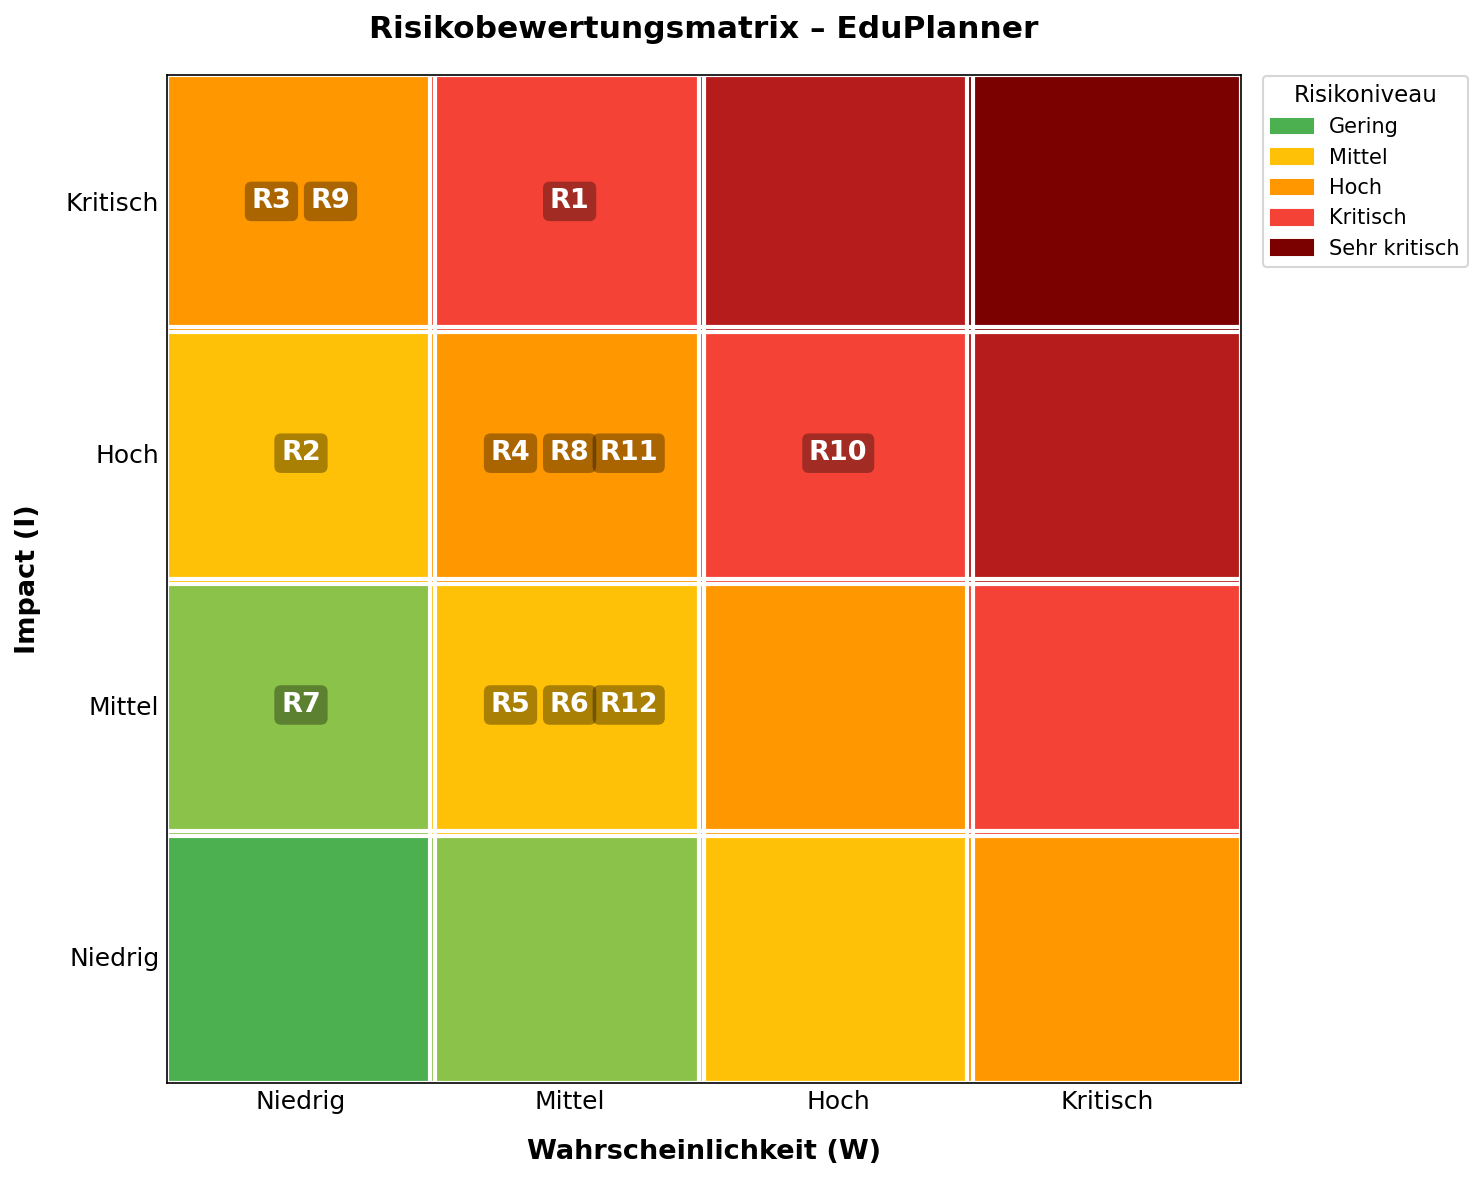
\includegraphics[width=\textwidth]{assets/RiskMatrix}
  \caption{\textit{Risikobewertungsmatrix: Wahrscheinlichkeit vs.\ Impact (R1--R12)}}
  \label{fig:RiskMatrix}
\end{figure}

\textbf{Bewertungsmatrix:} W~=~Wahrscheinlichkeit, I~=~Impact (jeweils: Niedrig / Mittel / Hoch / Kritisch)

\begin{longtable}{C{0.5cm} L{3.5cm} C{1.5cm} C{1.5cm} L{5.5cm}}
  \rowcolor{tableheader}
  \color{white}\textbf{\#} & \color{white}\textbf{Risiko} & \color{white}\textbf{W} & \color{white}\textbf{I} & \color{white}\textbf{Massnahme} \\
  \endfirsthead
  \rowcolor{tableheader}
  \color{white}\textbf{\#} & \color{white}\textbf{Risiko} & \color{white}\textbf{W} & \color{white}\textbf{I} & \color{white}\textbf{Massnahme} \\
  \endhead

  R1 & Race Condition bei Kapazitätsprüfung & Mittel & Kritisch & Optimistic Locking + DB-Unique-Constraint; Lasttests vor Go-Live. Validiert durch Q1. \\
  \rowcolor{tablegrey}
  R2 & RabbitMQ als Single Point of Failure & Niedrig & Hoch & 3-Node Quorum-Cluster; Monitoring; auto.\ Failover getestet. \\
  R3 & Ausfall des Identity Providers & Niedrig & Kritisch & SLA $\geq$ 99,9\,\%; Read-Only-Fallback; JWT-Cache (24\,h). \\
  \rowcolor{tablegrey}
  R4 & PII gelangt in Logs & Mittel & Hoch & Log-Scrubbing; PII-Scanner im CI (detect-secrets). \\
  R5 & Microservice-Overhead überfordert Team & Mittel & Mittel & Modularer Monolith als Fallback definiert; Entscheidung nach MVP. \\
  \rowcolor{tablegrey}
  R6 & Event-Schema-Änderungen brechen Consumer & Mittel & Mittel & Schema Registry evaluieren; nur additive Änderungen. \\
  R7 & Vendor Lock-in & Niedrig & Mittel & Cloud-agnostische Tools (K8s, PostgreSQL, RabbitMQ). \\
  \rowcolor{tablegrey}
  R8 & Key-Person-Abhängigkeit & Mittel & Hoch & Pair-Programming; ADRs als Gedächtnis; Architektur-Workshops. \\
  R9 & DB-Korruption / fehlgeschlagene Migration & Niedrig & Kritisch & Wöchentliche Restore-Tests; Flyway rückwärtskompatibel. \\
  \rowcolor{tablegrey}
  R10 & Team-Burnout \textit{[PM-Risiko]} & Hoch & Hoch & Hiring-Plan Q3; On-Call-Rotation max.\ 1~Wo/Monat. \textit{Anm.: primär Projektmanagement-Risiko, zur Diskussion als Lehrbeispiel.} \\
  R11 & Datenmigration bei Schema-Änderungen & Mittel & Hoch & Expand-Contract-Pattern; Zero-Downtime-Migrations via mehrphasiges Deployment; Staging-Test zwingend. \\
  \rowcolor{tablegrey}
  R12 & Budgetüberschreitung bei Lastspitzen & Mittel & Mittel & Cloud-Kosten variabel bei ungeplantem Traffic. Gegenmassnahme: Reserved Instances für Basisload (CHF~80 Einsparung = 10\,\% Puffer); HPA-Limits verhindern unkontrolliertes Scale-out; monatliches Capacity Review. \\
\end{longtable}

\subsection{Technische Schulden}

Technische Schulden bezeichnen bewusste architektonische Vereinfachungen, die kurzfristig Entwicklungsgeschwindigkeit ermöglichen, langfristig aber Wartungsaufwand oder Sicherheitslücken erzeugen können. Die nachfolgende Tabelle listet alle bekannten Schulden von EduPlanner, bewertet ihre Priorität und definiert einen konkreten Tilgungsplan. Schulden hoher Priorität sind für die nächsten Sprints eingeplant; Schulden niedriger Priorität werden spätestens vor dem v2.0-Release adressiert.

\begin{tabularx}{\textwidth}{C{0.5cm} L{3.5cm} C{1.8cm} X}
  \rowcolor{tableheader}
  \color{white}\textbf{\#} & \color{white}\textbf{Schuld} & \color{white}\textbf{Prio} & \color{white}\textbf{Erläuterung und Tilgungsplan} \\
  TS1 & Kein Service Mesh & Mittel & mTLS intern fehlt. Tilgung: Linkerd in v2.0 (ADR-007). \\
  \rowcolor{tablegrey}
  TS2 & Kein Contract Testing (Pact) & Hoch & API-Kompatibilität manuell koordiniert. Tilgung: Sprint~8. \\
  TS3 & E-Mail-Templates im Container & Niedrig & Änderungen erfordern Re-Deploy. Tilgung: Template-UI in v1.1. \\
  \rowcolor{tablegrey}
  TS4 & Fehlende Multi-Tenancy & Mittel & Single-Tenant (ADR-008). Tilgung: Schema-per-Tenant in v2.0. \\
  TS5 & Kein API-Versionsmanagement $>$~v1 & Niedrig & Tilgung: API-Versionierungsstrategie vor erstem externem API-Zugang -- geplant Sprint~12 (vor v1.0-Release). \\
  \rowcolor{tablegrey}
  TS6 & Keine Accessibility-Tests & Niedrig & WCAG~2.1 AA nicht geprüft. Tilgung: axe-core in v1.1. \\
  TS7 & Rate-Limiting nicht nach Rolle & Niedrig & Alle Rollen gleiche Limits. Tilgung: Kong-Konfig. Sprint~10. \\
\end{tabularx}